\begin{savequote}[8cm]
Alles Gescheite ist schon gedacht worden.\\
Man muss nur versuchen, es noch einmal zu denken.

All intelligent thoughts have already been thought;\\
what is necessary is only to try to think them again.
  \qauthor{--- Johann Wolfgang von Goethe \cite{von_goethe_wilhelm_1829}}

Dancing is more important. --- Pauli
\end{savequote}

\chapter{\label{ch:2-neutrinos}The Field of Neutrinos}
\minitoc

As a neutrino physicist, an overall understanding of the field is necessary.

\section{The History}
\subsection{The Past}
The field of neutrino has a dramatic opening that many know of - in a letter~\cite{Pauli:1930pc} from Wolfgang Pauli to the Radioactivity conference in 1930, which he did not attend in person as he was rumoured to be going for a dance instead. 
The letter was proposing a solution to the then very puzzling problem of $\beta$ decay.
It was thought of a two body decay, where the heavier nucleus decay to a lighter nucleus and an electron, which carries away a well-definied amount of energy due to the mass difference between the parent and daughter nucleus.  
However, the measured electron energy spectrum was a wide distribution rather than the fixed value expected. 
In his letter, Pauli postulated a third but un-detected particle in the decay that shared the energy budget with electron so that the sum of the third particle energy and the electron energy is equal to the fixed value expected, but not the electron energy alone. 
Originally, he coined this particle the ``neutron'', but this name did not stick and was given to the now known neutron discovered by James Chadwick in 1932.
The present name, ``neutrino'', was later coined by Edoardo Amaldi in a conversation with Enrico Fermi, who later published the seminal paper on his theory of beta decay in 1934~\cite{Fermi:1934hr}, laying the solid theoretical foundation for subsequent experimental work.
However, the cross section for neutrino interaction is estimated to be so small and hence extremely difficult to observe that even Pauli lamented, 
``I have done a terrible thing. I have postulated a particle that cannot be detected.''

It was such a formidable task that Frederick Reines even proposed to use the atomic bomb  as the neutrino source to have an intense source of neutrino for detection.
Fortunately, Reines and his collaborator, Clyde Cowan, discovered that the delay of the signal of the neutron capture from the signal of the annihilation between electron and positron, the product of the anti-neutrino interaction, is distinct and could be utilized to significantly reduce backgrounds such that a less intense (dangerous) source of (anti)neutrino can be used.
It was not until about 26 years after the postulation of neutrino that it was directly detected in the Cowan-Reines experiment at the Savannah River plant in 1956~\cite{Cowan:1956rrn}. 
The detector was mainly composed of $1400$ litres of liquid scintillator and $200$ litres of Cadium-loaded water as target and neutron capturer.
This remarkable achievement was recognised with a Nobel Prize in 1995.

After the Cowan-Reines experiment, the existence of neutrion is beyond doubt and the field of neutrino phsyics developed rapidly. 

There were two naturally complementary directions for development.
One is to build larger and more advanced detectors to measure the existing neutrino sources, for example, the solar neutrinos, the reactor neutrinos, the atmospheric neutrinos and others.
The other is to include the neutrino production as part of the experiment, which becomes the field of accelerator neutrinos.

Roughly about the same time, Raymond Davis was also working in the Savannah River plant, using the inverse beta decay of chlorine to argon, suggested by Pontecorvo~\cite{Pontecorvo:1946mv}, to detect neutrinos.
His experiment measured a $20$ times smaller crosss section for anti-neutrino than for neutrino in the inverse beta decay turning cholrine into argon, providing evidence for neutrino antineutrino being different particles~\cite{Davis:1959pba}.
Later he applied the same technique to measure the solar neutrino flux with a detector of the size of $378,000$ litres at the Homestake Mine~\cite{Davis:1964zz}, sufficient to detect solar neutrinos based on the Standard Solar Model calculation done by John Bahcall~\cite{Bahcall:1964ya}. 
It was to everyone's surprise that the Homestake experiment only observed about $1/3$ of the expected flux~\cite{Davis:1968}, a discrepancy known as the solar neutrino problem.
Davis and Bahcall did meticulous checks on their results and found no errors large enough to explain the discrepancy.
This phenonemon has sparked many efforts, both experimentally and theoretically, to resolve the observed discrepancy.
The solution we now know consists of neutrino oscillation and the Mikheyev-Smirnov-Wolfenstein (MSW) effect~\cite{Wolfenstein:1977ue,Mikheyev:1985zog}.
The idea of neutrino oscillation was actually proposed even before the solar neutrino problem by Pontecorvo in 1957~\cite{Pontecorvo:1957qd} and completed by Maki, Nakagawa and Sakata in 1962~\cite{Maki:1962mu}.
However, it was just one of the possible solutions back then among many other theories.
Papers on the other piece of the solution, the MSW effect, was published in the 1980s.
The combined solution, the large-mixing-angle MSW solution, provided an attractive answer to the solar problem.
Subsequent experiments, such as Kamiokande, a $3,000,000$-litre water cherenkov experiment lead by Masatoshi Koshiba~\cite{Kamiokande-II:1989hkh}, GALLEX~\cite{GALLEX:1998kcz} and SAGE~\cite{SAGE:1999nng}, confirmed the solar neutrino deficit.
The definitive evidence came in 2001, when the Sudbury Neutrino Observatory (SNO) experiment, with a $1,000,000$-litre heavy water Cerenkov detector, published its result~\cite{SNO:2001kpb}, directly showing that the observed deficit of electron neutrino is oscillated into other flavours.
In the next year, Davis and Koshiba promptly received a Nobel Prize in Physics.
Meanwhile, in 1998, the upgrade of Kamiokande, the Super-Kamiokande ($50,000,000$-ton water Cerenkov detector), reported the observation of neutrino oscillation in atmospheric neutrinos~\cite{Super-Kamiokande:1998kpq}.
Takaaki Kajita (Super-Kamiokande) and Arthur McDonald (SNO) shared a Nobel prize for their work on neutrino oscillation in 2015.

Along the other development route, Pontecorvo suggested the possibility of using accelerated proton hitting on targets to produce mesons that decay to produce a beam of neutrinos in 1959~\cite{Pontecorvo:1959sn}.
A year later, a similar proposal was made independently by Mark Schwartz~\cite{Schwartz:1960hg} to use the accelerator-produced neutrinos to address another puzzle at that time, if the muon neutrino is the same as the electron neutrino.
Schwartz and his collaborators, which included Leon Lederman and Jack Steinberger, used the Alternate Gradient Synchrotron at the Brookhaven National Laborarory to perform the first accerlator neutrino beam. 
The neutrino interaction was recorded by a $10$-ton spark chamber, which were able to reconstruct clear muon tracks from the interaction.
In 1962, the collected data proved that muon neutrinos are distinct from electron neutrinos~\cite{Danby:1962nd}.
Schwartz, Lederman and Steinberger were awarded the Nobel Prize in 1988.
For the subsequent decades, the accelerator neutrinos were used in turn to help progress the more general field of particle physics due to the unique nature of neutrino scattering.
For instance, neutral current interaction was first observed by the Gargamelle bubble chamber at CERN using a beam of neutrinos~\cite{GargamelleNeutrino:1973jyy}.
High energy neutrino beams were also deployed to test the electroweak theory and study the nucleon structure by the CDHS experiment at CERN~\cite{Schlatter:2015nxk}.

The field has entered a phase of precision measurement that will be illustrated in the next subsection.
The two complementary development routes in the past has combined in long-baseline experiments to elucidate the few remaining questions in the field.

% To better appreciate the historical progress of neutrino physics, it is clearer to put it in the perspective of the overall development of particle physics.

% Electron was discovered by J.J. Thomson in 1897.
% Proton was discovered by Rutherford in 1917.
% Neutron was discovered by Chadwick in 1932.
% Paul Dirac published the famous Dirac equation in 1928, predicting the existence of the positron, the anti-particle of the electron, which was discovered by Carl Anderson in 1932.
% Beta decay was discovered by Lise Meitner and Otto Hahn in 1938 to be a weak interaction process, where a neutron decays to a proton, an electron and an anti-neutrino.
% The muon was discovered by Carl Anderson in 1936, which was initially thought to be the Yukawa particle responsible for the strong nuclear force.

% ``Weak interaction'' is first coined by Enrico Fermi in 1933 to describe the force responsible for beta decay. <CHECK>
% On the theoretical front, Fermi proposed a theoretical solution to the beta decay in 1934.

% In 1954, CN Yang and Robert Mills published the seminal paper on non-abelian gauge theory, laying the foundation for the Standard Model.
% In 1960s and 1970s, rapid progress was made in the unifications of the electromagnetic and weak interactions, leading to the Glashow-Salam-Weinberg (GSW) model, who shared the Nobel Prize in Physics in 1979. 
% The discovery of the W and Z bosons at CERN in 1983.

% It was suggested by Markov [65], Pontecorvo [66], and Schwartz [67] to use proton accelerators to produce high energy
% neutrino beam from pion decays to perform experiments like:
% nu+n->mu+n
% etc
% The experiments performed at the Brookhaven National Laboratory (BNL) by Danby et al. [71] and later at
% CERN by Bienlein et al. [72] 
% observed only muon but never elec tron, confirming numu and nue are different (1962)

% 1965 BNL introducted the POT idea as a measure of the neutrino flux

% Tau in 1975
% the existence of a new flavor of
% neutrinos ντ was proposed, which was observed much later in the DONUT experiment [74,75] in 2000 at the Fermilab

% It was Fermi [3,4] and Perrin [5] who first discussed the determination of the neutrino mass from the study of the end-point spectrum of beta decay.

\subsection{The Present}
With neutrino oscilaltion finally confirmed, the field of neutrino physics has a fruitful past and a clear theoretical framework laid out.
The present task for the field is the precise measurement of the parameters in the theoretical framework, namely the neutrino masses and the PMNS matrix elements.
The measurements given in this section follows from the latest Particle Data Group release~\cite{ParticleDataGroup:2024cfk}.

The mass electron neutrino can be studied by investigating the shape of the high energy tail of the electgron spectrum in tritium beta decay, a method proposed in Fermi's theory paper on $\beta$-decay~\cite{Fermi:1934hr} and independently by Francis Perrin~\cite{Perrin1933}.
The KATRIN experiment employs this method and produces one of the most stringent upper-bound, $0.8\ev$ with $90\%$ confidence level~\cite{KATRIN:2021uub}.
There are other methods to extract the neutrino mass, such as from cosmological observation~\cite{Brieden:2022lsd}, but as this thesis focuses on neutrino oscillation, this will not be elaborated for conciseness.

As neutrino oscillation depends on the mass difference squared as well, oscillation experiments are able to measure the neutrino masses indirectly through the mass differences in addition to the PMNS matrix elements.
Contrary to the electron neutrino mass measured from $\beta$-decay, the mass differences measured in oscillation experiments are the differences between the neutrino mass eigenstates.
The general structure of the mass eigenstates is that there is a small difference between $m_2$ and $\m_1$, but $m_3$ is either much smaller or larger than $m_2$ and $m_1$.
The relation between $m_3$ and the others is the mass hierachy problem.
The case where $m_3$ is the largest is called the Normal Ordering (NO), and the case where $m_3$ is the smallest is the Inverted Ordering (IO).
The KamLAND collaboration performed a global fit of data sets across several types of neutrino experiments in 2013, leading to the measurement of $\delmtwoo=7.53^\pm0.18~\times 10^{-5}~\ev$~\cite{KamLAND:2013rgu}.
Note that this difference is not the absolute value as it is known that $m_2>m_1$.
As for $\delmthro$, the estimation is produced from a global fit of accerlator, reactor and atmospheric data by PDG, giving $\delmtwoo=2.455^\pm0.028~\times 10^{-3}~\ev$ (NO) and $\delmtwoo=-2.455^\pm0.028~\times 10^{-3}~\ev$ (IO).

The specific meaning of the parameters in the PMNS matrix will be illustrated later in Sec.~\ref{subsec:oscilaltion}, while the respective measurements are first given here without breaking the flow.
The PMNS matrix can be parameterized by three mixing angles, namely $\totwo$, $\tothr$ and $\ttthr$, and a CP violation phase, $\dcp$.
The current best estimate of $\totwo$ is given by a fit of the KamLAND measurement and solar measurements in 2016, producing $\sin^2(\totwo)=0.307^{+0.013}_{-0.012}$.
The estimation of $\ttthr$ is done by the PDG using accerlator and atmospheric neutrino data~\cite{ParticleDataGroup:2024cfk}, leading to $\sin^2(\ttthr)=0.553^{+0.016}_{-0.024}$ (IO) and $\sin^2(\ttthr)=0.558^{+0.015}_{-0.021}$ (NO).
The last mixing angle, the average of $\tothr$ is obtained by PDG using accelerator and reactor data, giving $\sin^2(\tothr)=2.19\pm0.07$.
The last parameter, $\dcp$, is the least well measured.
The PDG average of exiting accerlator and atmospheric data gives $\dcp=1.19\pm0.22$ in radian.

From being completely unknown to precisely measured, neutrino oscillation is now a well-understood phenonemon except the mass ordering and the extent of CP violation, which is the pressing goal of the present and future LBL neutrino experiments.
 
\subsection{The Plans}
To eluciate the remaining questions in neutrino physics, new experiments are planned or under construction and existing experiments are undergoing upgrades.
The sub-section will only briefly some of them and it is not meant to be an exhaustive review.

The successor of the Daya bay experiment, which produced one of the most precise measurements of $\tothr$, the JiangMen Underground Neutrino Observatory (JUNO), is set to start operation in summer 2025~\cite{ScienceNews2025}.
Located near the Yangjiang and Taishan nuclear power plants, JUNO has a $20,000$-ton liquid scintillator.
It is projected to determine the mass ordering with $3~(3.1)\sigma$ significance for NO (IO) in $6.7$ years of data taking~\cite{Paoloni:2024atc}.

The successor of the Super-K experiment, the Hyper-Kamiokande (Hyper-K)~\cite{Hyper-Kamiokande:2018ofw}, is under construction and is expected to operate in 2027.
Hyper-K is a $258,000$-ton water Cerenkov detector, about $8$ times of the size of tis predecessor, Super-K.
It uses the same beamline as the T2K experiment and measures the electron neutrino appearance to determine $\dcp$.
With $10$-year data taking, it is projected to exclude CP conservation to $5\sigma$ for more than $60\%$ of true $\dcp$ values and to $3\sigma$ for $75\%$ of $\dcp$ values assuming the systematic uncertainties are controlled at $2.7\%$~\cite{Jesus-Valls:2024ady}.

Another large scale LBL neutrino is the Deep Underground Neutrino Experiment (DUNE)~\cite{DUNE:2016hlj,DUNE:2015lol,DUNE:2016evb,DUNE:2016rla,DUNE:2021tad}.
Its far detector consists of four $17,000$-ton Liquid Argon Time Projection Chamber (LArTPC) and it has a beamline of $1300$~km, which enables it to be highly sensitive to the mass ordering as well.
With the novel LArTPC technology, it is expected to reach $5\sigma$ for the mass ordering with 3-year data taking and reach $3\sigma$ for $75~\%$ of $\dcp$ values with about $15$ years of data taking~\cite{Gil-Botella:2024duf}.
There is no clear estimation of starting time for DUNE yet, but the test experiment for its far detector, the ProtoDUNE experiment, has operated for more than $2$ years at CERN.

In the projected sensitivity of these future experiments, the importance of reducing systematic uncertainties cannot be over-emphasized as results obtainable with years of data taking would need decades instead if the systematic uncertainties do not reach the required level.
This is exactly why T2K is upgrading its near detector to better understand neutrino interactions to reduce systemtics, which is exactly what this thesis is about.

Besides the measurement of the known parameters, there are also a plethora of beyond the Standard Model searches both at existing and future experiments.
Moreover, there has been impressive progress on utilising neutrino for cosmological observation by experiments, such as IceCUBE.
Although they are not elaborated in this thesis, they represent the highly exciting development of the field.
From the $1400$-litre liquid scintillator detector in the Cowan-Reines experiment to the $1,000,000$-litre heavy water Cerenkov detector of SNO and to the $258,000,000$-litre water Cerenkov detector of Hyper-K, the field of neutrino physics has grown rapidly. 
From being the most elusive particle, which was thought never possible to detect, to a sophisticated understanding of neutrino oscilaltion, our understanding of the properties of neutrino has improved drastically.
With the incredible experiments in plan and running, it is promising that a definitive measurement of all the neutrino properties is reachable, and its results will be profound and shed light on new physics direction.

\section{The Theory}
The main goal of neutrino experiments is to measure all neutrino properties, including the mass, mixing angles, and the CP violation parameter, $\dcp$. 
The mixing angles and $\dcp$ fully describes neutrino oscillation, while the mass is the reason why neutrino oscillation happens.
Hence, these parameters will be better illustrated in the following Sec.~\ref{subsec:oscillation} in the context of the theoretical framework of neutrino oscillation.
As only products from neutrino interaction are detected in experiments, to achieve the said goal, a good understanding of neutrino interaction is necessary.
Hence, a brief overview of neutrino interaction is given in Sec.~\ref{subsec:interaction}.

\subsection{Oscillation}
\label{subsec:oscillation}
Neutrinos come in three flavours: electron neutrino ($\nu_e$), muon neutrino ($\nu_\mu$), and tau neutrino ($\nu_\tau$).
The different flavours of neutrinos will only produce the corresponding lepton in weak interaction, so they are eigenstates of the weak interaction.
However, neutrinos propagate through space as mass eigenstates, $\nu_1$, $\nu_2$, and $\nu_3$.
The reason for neutrino oscillation to occur is two-fold.
One is beacuse the mass eigenstates do not have a simple one-to-one correspondence with the weak eigenstates. 
They are a superposition of the weak eigenstates and vice versa.
The other is beacuse these mass eigenstates have different masses.
Neutrinos are created as flavour eigenstates in weak interaction, but they propagate as a linear combination of mass eigenstates, which propagate with different phase velocities due to their different masses.
Hence, throughout the propagation, the linear combination of mass eigenstates is changing constantly, leading to a changing superposition of flavour eigenstates, and thus, neutrino oscillation.

To be more specific, the matrix describing the mixing of mass eigenstates to flavour eigenstates is the PMNS matrix.
It is conventionally parameterized as follows:

\begin{equation}
U_{\text{PMNS}} = 
\begin{pmatrix}
1 & 0 & 0 \\
0 & c_{23} & s_{23} \\
0 & -s_{23} & c_{23}
\end{pmatrix}
\begin{pmatrix}
c_{13} & 0 & s_{13} e^{-i\dcp} \\
0 & 1 & 0 \\
-s_{13} e^{i\dcp} & 0 & c_{13}
\end{pmatrix}
\begin{pmatrix}
c_{12} & s_{12} & 0 \\
-s_{12} & c_{12} & 0 \\
0 & 0 & 1
\end{pmatrix}
\end{equation}
where $c_{ij} = \cos\theta_{ij}$ and $s_{ij} = \sin\theta_{ij}$, and $\dcp$ is the CP violation phase.
The angles, $\theta_{ij}$, are the mixing angles. 
Using the PMNS matrix, the flavour eigenstates can be expressed in terms of the mass eigenstates as follows:
\begin{equation}
\begin{pmatrix}
\nu_e \\
\nu_\mu \\
\nu_\tau
\end{pmatrix}
=
U_{\text{PMNS}}
\begin{pmatrix}
\nu_1 \\
\nu_2 \\
\nu_3
\end{pmatrix}
\end{equation}
To keep a close focus on the development of the theoretical idea, detailed derivations are rendered to the Appendix~\ref{app:oscillation}, and only important results are included here for elaboration.
Due to the small neutrino masses, the mass eigenstate, with mass $m_i$, acquires a phase approximately of
\begin{equation}
  \ket{\nu_i(L)} = e^{-i \frac{m_i^2L}{2E}} \ket{\nu_i(0)},
\end{equation}
after travelling a distance $L$ with energy $E$.
Hence, the probability of a neutrino of flavour $\alpha$ at creation to be detected as a neutrino of flavour $\beta$ after travelling a distance of $L$ is given by
\begin{array}{rl}
  P_{(\alpha \to \beta)} &= \left|\braket{\nu_\beta | \nu_\alpha(L)} \right|^2 = \left| \sum_i U_{\alpha i} U^*_{\beta i} e^{-i \frac{m_i^2L}{2E}} \right|^2 \\
  &= \delta_{\alpha\beta} - 4 \sum_{i>j} \text{Re} \left( U_{\alpha i} U^*_{\beta i} U^*_{\alpha j} U_{\beta j} \right) \sin^2 \left( \frac{\Delta m^2_{ij} L}{4E} \right) \\
  &+ 2 \sum_{i>j} \text{Im} \left( U_{\alpha i} U^*_{\beta i} U^*_{\alpha j} U_{\beta j} \right) \sin \left( \frac{\Delta m^2_{ij} L}{2E} \right),
\end{array}
where $\delta{\alpha\beta}$ is the Kronecker delta, $U_{\alpha i}$ is the element of the PMNS matrix, and $\Delta m^2_{ij} = m_i^2 - m_j^2$.
This result shows that the oscillation probability depends on the mixing angle through the PMNS matrix elements and on the mass difference and neutrino energy through the sine terms.
For brevity, the dependence on the sine terms can be characterised by a phase angle,
\begin{equation}
  \label{eq:osc-phase}
  \Delta_{ij} = \frac{\Delta m^2_{ij} L}{2E} \approx 1.27 \frac{\Delta m^2_{ij} \text{eV}^2 L \text{km}}{E \text{GeV}},
\end{equation}
where the oscillation is maximal when $\Delta_{ij} = \pi / 2$.
These results can be used to better understand how the various parameters are measured in different types of neutrino experiments.
The different sensitivies of these experiments are due to the relatively large difference in the mixing angles and the mass differences.
The latest values for the neutrino parameters based on Ref.~\cite{Capozzi:2021fjo,ParticleDataGroup:2024cfk} are given in Table~\ref{tab:neutrino-parameters}, which shows that the magnitude of $\delta_{21}$ is much smaller than that of $\delta_{31}$.
Unlike the CKM matrix, where all mixing angles are small, only $\theta_{13}$ is small while the other two angles are considerably larger, suggesting significant mixing.

\begin{table}[h]
  \centering
  \begin{tabular}{c|c|c}
    Parameter & Value & Sensitive Experiment\\
    \hline
    \hline
    $\Delta m^2_{21}~(\ev^2)$ & $7.36^{+0.16}_{-0.15} \times 10^{-5}$ & Reactor and solar \\
    $|\Delta m^2_{31}|~(\ev^2)$ & $2.448^{+0.023}_{-0.031} \times 10^{-3}$ & Atmospheric \\
    $\theta_{12}$ ($\deg$) & $33.40^{+0.80}_{0.82}$ & Reactor and solar \\
    $\theta_{23}$ ($\deg$)       & $42.4^{+1.0}_{0.9}$ & Atmospheric\\
    $\theta_{13}$ ($\deg$)       & $8.59^{+0.13}_{0.12}$ & Reactor and solar \\
    $\dcp$ ($\deg$) & $223^{+32}_{-23}$   & Accelerator \\
    \hline
  \end{tabular}
  \caption{The latest values for the neutrino parameters.}
  \label{tab:neutrino-parameters}
\end{table}



\subsubsection{Atmospheric neutrinos}
  Atmospheric neutrinos are mostly muon neutrinos produced from decays of mesons produced by cosmic rays interacting with the atmosphere.
  The neutrino energy is typically of the order of $1~\gev$, while the distrance travelled has a range of $O(10^2)$ to $O(10^4)~\km$.
  Substituting these numbers into \Eq.~\ref{eq:osc-phase}, $\Delta_{23}$ is of the order of $O(10^(-2))$ to $O(1)$, while $\Delta_{21}$ is of the order of $O(10^(-3))$ to $O(10^(-1))$.
  Hence, oscillation is much more prominent in the $\nu_\mu \to \nu_\tau$ channel than in the $\nu_\mu \to \nu_e$ channel.
  This is why atmospheric neutrino experiments are sensitive to $\theta_{23}$ and $\Delta m^2_{32}$, which are sometimes referred to as the atmospheric mixing angle and mass difference, respectively.

\subsubsection{Reactor neutrinos}
  Reactor neutrinos are mostly electron antineutrinos produced from nuclear fission in the power plants.
  The neutrino energy is typically of the order of $1~\mev$.
  Unlike the atmospheric neutrino measurement, detectors can be placed at various locations to measure different parameters.
  Thus, it is easier to discuss reactor neutrino oscillation by introducing the oscillation length variable given as:
  \begin{equation}
    \label{eq:osc-length}
    L_{\text{osc}} = \frac{4\pi E}{\Delta m^2} = 2.48 \frac{E \text{MeV}}{\Delta m^2 \text{eV}^2} \text{m},
  \end{equation}
  which corresponds to one complete period of neutrino oscillation.
  Substituting the reactor neutrino energy into Eq.~\ref(eq:osc-length), one gets $L_{\text{osc}} = O(10^2)~\km$ for $\delmtwoo$ and $L_{\text{osc}} = O(1)~\km$ for $\delmthro$. 
  Hence, by placing detectors kilometers away from the power plants, reactor neutrino experiments offer the unique opportunity to measure $\tothr$ and $\delmthro$, which are sometimes referred to as the reactor mixing angle and mass difference, respectively.
  Additionally, placing detectors at around $O(100)~\km$ away from the power plants allows the measurement of $\delmtwoo$.

  \subsubsection{Solar neutrinos}
  Solar neutrinos are mostly electron neutrinos produced from nuclear fusion in the sun.
  The majority of solar neutrinos have energies below $1~\mev$, except those from the $^8$B decay, which have energies up to $15~\mev$.
  The distance travelled by solar neutrinos is of the order of $O(10^8)~\km$.
  Substituting these values into Eq.~\ref{eq:osc-length}, one gets $L_{\text{osc}} = O(10^4)~\m$ for $\delmtwoo$ and $L_{\text{osc}} = O(10^3)~\m$ for $\delmthro$.
  Both are much smaller than the average distance travelled, so to observe the clear oscillatory pattern like in other neutrino experiments, the exact distance travelled by the individual neutrino needs to be known with an incredibly high precision, which is beyond the current detection capability.
  Fortunately, the average oscillation result can still be measured by the total survival rate of the electron neutrinos.
  
  On top of the usual neutrino oscillation, there is another important phenonemon at play in the solar neutrino measurements, which is the Mihheev-Smirnov-Wolfenstein (MSW) effect~\cite{Wolfenstein:1977ue,Mikheyev:1985zog}.
  A full discussion on the MSW effect is beyond the scope of this thesis.
  Simply put, the MSW effect is the modification of the mixing parameters due to the presence of electrons in matter. 
  This modification can enhance or suppress the oscillation probability depending on the mass difference and the electron density.
  Approximately, the required electron density is proportional to the mass difference squared and inversely proportional to the neutrino energy.
  Hence, the lower the neutrino energy or the larger the mass difference, the higher the electron density is required to modify the oscillation probability.
  Due to the considerably larger $\delmthro$, for almost the whole energy range of solar neutrinos, the electron density in the Sun is not sufficient to modify the mixing between $\nu_1$ and $\nu_3$.
  As for the relatively smaller $\delmtwoo$, the electron density is high enough to significantly modify the mixing between $\nu_1$ and $\nu_2$ for the high energy neutrinos from the $^8$B decay.
  The resultant impact on these high energy electron neutrinos is an alteration of its composition of the mass eigenstates such that when they leave the surface of the Sun, they are mainly composed of $\nu_2$, a considerably larger fraction than the unmodified composition.
  The MSW effect is demonstrated when different experiments measure solar neutrinos with different energies and observe a different survival rate of electron neutrinos.
  The absolute survival rates are sensitive to $\totwo$ and $\tothr$ for the low energy region and the high energy region, respectively.


\subsubsection{Accelerator neutrinos}
  In accelerator neutrino experiments, there is relatively greater freedom than in other types of neutrino experiments as both the neutrino source and the detector are designed to optimize osicllation.
  This section uses T2K as an example, but the underlying principles are common to all LBL experiments.
  More details of the T2K experiment will be illustrated in Chapter~\ref{ch:t2k}.

  Neutrinos are produced in accelerators by bombarding protons on some form of target, carbon in the case of T2K, to produce an abundance of mesons.
  The charged mesons can be redirected to point in the desired direction using sophisticated magnetic horn.
  Besides directionality, the magnetic horn can also select the mesons of the desired charge.
  For example, positive (negative) pions can be focused if a beam of muon (anti-)neutrinos are needed.
  It is this control over the neutrino source that enables accelerator experiments to measure $\dcp$.
  As the neutrino energy from the meson decay is angular dependent, it is possible to obtain a beam of neutrinos with different energy spread by varying the angle of the detector respective to the beam direction. 
  T2K places its detectors at $2.5\deg$ off-axis to obtain a neutrino beam narrow in energy distribution with a peak at $0.6~\gev$.
  According to Eq.~\ref{eq:osc-phase}, to achieve maximal oscillation, the far detector needs to be placed at a length of approximately $300$~km from the source for the larger mass difference, i.e. $\delmthrt\approx\delmthro\approx2.5\times10^{-3}eV$.
  This is why accelerator measurments are sensitive to $\tttthr$.
  By analysing oscillation in the neutrino mode and in the anti-neutrino mode, T2K is able to extract the best-fit value of $\dcp$ that could describe the collected data~\cite{T2K:2019bcf}.
  However, the current measurement is heavily limited by statistics and thus has large uncertainties.
  In the Hyper-K era, the statistics is expected to increase significantly, and to maximize the potential of the measurement, a commensurate reduction in systematic uncertainties is of paramount importance.
  This leads us naturally to the discussion of one of the major systemtics in neutrino experiments, neutrino interactions.

\subsection{Interaction}
\label{subsec:interaction}

The underlying theory for neutrino oscillation is straightforward, and the parameters to be measured are clear, but the experimental determination of these parameters is challenging.
Due to the weak interaction of neutrinos, they cannot be detected directly.A
All neutrino measurements are based on the detection of the particles produced in the neutrino interaction.
Therefore, to extract the desired neutrino oscillation parameters with a high precision, a good understanding of neutrino interactions is crucial.
This chapter provides the basic understanding of neutrino interactions necessary for the interpretation of the analyses presented in the subsequent chapters.

\subsubsection{nu-quark}
The most fundamental interaction between a neutrino and matter is the weak interactions between the neutrino and a quark, the Feynman diagrams for which are shown in Fig.~\ref{fig:nu-q-feyn}.

\begin{figure}[h]
  \centering
  \begin{subfigure}[b]{0.45\textwidth}
    \centering
    \begin{tikzpicture}
      \begin{feynman}
        \vertex (a) {\(\nu_\ell\)};
        \vertex [right=of a] (b);
        \vertex [right=of b] (c) {\(\ell\)};
        \vertex [below=of b] (d);
        \vertex [left=of d] (e) {\(q\)};
        \vertex [right=of d] (f) {\(q'\)};
        
        \diagram* {
          (a) -- [fermion] (b) -- [fermion] (c),
          (b) -- [boson, edge label=\(W\)] (d),
          (e) -- [fermion] (d) -- [fermion] (f),
        };
      \end{feynman}
    \end{tikzpicture}
    \caption{Charge current interaction.}
    \label{fig:cc-interaction}
  \end{subfigure}
  \hfill
  \begin{subfigure}[b]{0.45\textwidth}
    \centering
    \begin{tikzpicture}
      \begin{feynman}
        \vertex (a) {\(\nu_\ell\)};
        \vertex [right=of a] (b);
        \vertex [right=of b] (c) {\(\nu_\ell\)};
        \vertex [below=of b] (d);
        \vertex [left=of d] (e) {\(q\)};
        \vertex [right=of d] (f) {\(q\)};
        
        \diagram* {
          (a) -- [fermion] (b) -- [fermion] (c),
          (b) -- [boson, edge label=\(Z\)] (d),
          (e) -- [fermion] (d) -- [fermion] (f),
        };
      \end{feynman}
    \end{tikzpicture}
    \caption{Neutral current interaction.}
    \label{fig:nc-interaction}
  \end{subfigure}
  \caption{Feynman diagrams for neutrino interactions with a quark.}
  \label{fig:nu-q-feyn}
\end{figure}
More specifically, Fig.~\ref{fig:cc-interaction} is mediated by the $W$ boson and the neutrino is converted to a charged lepton, while Fig.~\ref{fig:nc-interaction} is mediated by the $Z$ boson and the neutrino remains a neutrino.
The former is the charged current (CC) interaction, while the latter is the neutral current (NC) interaction.
Following the Feynman diagram, it is straightforward to write down the amplitude for the interaction.
The amplitude for the CC interaction is given by:
\begin{equation}
  \mathcal{M}_{\text{CC}} = \frac{g^2}{2} \bar{u}_\ell(p') \gamma^\mu (1 - \gamma^5) u_\nu(p) \frac{-i g_{\mu\nu}}{q^2 - M_W^2} \bar{u}_q(k') \gamma^\nu (1 - \gamma^5) u_q(k),
\end{equation}
where $g$ is the weak coupling constant, $u_\ell$ and $u_\nu$ are the spinors for the outgoing lepton and incoming neutrino, respectively, $u_q$ are the spinors for the quarks, $q$ is the momentum transfer, and $M_W$ is the mass of the $W$ boson.
This interaction takes place only when the neutrino possesses high enough energy <how high?> to probe inside the nucleon and interact with the quarks.
The product quark will hadronize and produce a jet of particles.
This type of interaction is refered to as deep inelastic scattering (DIS).
DIS is highly complicated, but no so relevant for this thesis, so will not be discussed further.
More details can be found in reviews, such as Ref.~\cite{}. <DIS review>

\subsubsection{nu-nucleon}
At the T2K beam energy, the predominant fraction of the neutrinos do not possess the energy to probe inside the nucleon, but rather interact with the nucleon as a whole.
Depending on the specific neutrino energy, the interaction can be classified as quasi-elastic (QE), resonance, or deep inelastic scattering (DIS).

  \subsubsubsection{QE}
  Although at the quark level, the interaction appears to the same as the $\nu$-quark interaction shown in Fig.~\ref{fig:nu-q-feyn}, the interacted quark cannot be treated as independent, but rather as part of a nucleon.
  Hence, the effective $\nu$-nucleon interaction feynman diagram is shown in Fig.~\ref{fig:nu-n-feyn}.
  \begin{figure}[h]
    \centering
    \begin{subfigure}[b]{0.45\textwidth}
      \centering
      \begin{tikzpicture}
        \begin{feynman}
          \vertex (a) {\(\nu_\ell\)};
          \vertex [right=of a] (b);
          \vertex [right=of b] (c) {\(\ell\)};
          \vertex [below=of b] (d);
          \vertex [left=of d] (e) {\(N\)};
          \vertex [right=of d] (f) {\(N'\)};
          
          \diagram* {
            (a) -- [fermion] (b) -- [fermion] (c),
            (b) -- [boson, edge label=\(W\)] (d),
            (e) -- [fermion] (d) -- [fermion] (f),
          };
        \end{feynman}
      \end{tikzpicture}
      \caption{Charge current interaction.}
      \label{fig:cc-interaction-n}
    \end{subfigure}
    \hfill
    \begin{subfigure}[b]{0.45\textwidth}
      \centering
      \begin{tikzpicture}
        \begin{feynman}
          \vertex (a) {\(\nu_\ell\)};
          \vertex [right=of a] (b);
          \vertex [right=of b] (c) {\(\nu_\ell\)};
          \vertex [below=of b] (d);
          \vertex [left=of d] (e) {\(N\)};
          \vertex [right=of d] (f) {\(N\)};
          
          \diagram* {
            (a) -- [fermion] (b) -- [fermion] (c),
            (b) -- [boson, edge label=\(Z\)] (d),
            (e) -- [fermion] (d) -- [fermion] (f),
          };
        \end{feynman}
      \end{tikzpicture}
      \caption{Neutral current interaction.}
      \label{fig:nc-interaction-n}
    \end{subfigure}
    \caption{Feynman diagrams for neutrino interactions with a nucleon.}
    \label{fig:nu-n-feyn}
  \end{figure}
  The leptonic current remains the same, but the hadronic current is now a nucleon current instead of a quark current.
  Hence, the hadronic current is much more complicated and and comprises of several form factors, which paramterize our understanding of the nucleon structure.
  For instance, the hadronic current for the CC interaction is given by:
  \begin{equation}
    \mathcal{M}_{\text{CC}} = \frac{G_F}{\sqrt{2}} \bar{u}_\ell(p') \gamma^\mu (1 - \gamma^5) u_\nu(p) \bar{u}_N(k') \left[ F_1(q^2) \gamma_\mu + F_2(q^2) \frac{i \sigma_{\mu\nu} q^\nu}{2M} + F_A(q^2) \gamma_\mu \gamma^5 + F_P(q^2) \frac{q_\mu \gamma^5}{m_\pi} \right] u_N(k),
  \end{equation}
  where $G_F$ is the Fermi constant, $F_1$, $F_2$, $F_A$, and $F_P$ are the form factors, $M$ is the nucleon mass, and $m_\pi$ is the pion mass.
  The derivation is complicated and beyond the scope of this thesis. 
  More details can be found in Ref.~\cite{LlewellynSmith:1978te}.
  It is however important to note that $F_1$ and $F_2$ are the vector form factors, which can be extracted from the electron scattering measurements, and $F_P$ is the pseudoscalar form factor, which can be related to $F_A$, the axial form factor, through the Partially Conserved Axial Current Hypothesis (PCAC) .
  Hence, the axial form factor is unique to neutrion experiments and can only be extracted from past measurements.
  Fig.~\ref{fig:cc0pi} shows an event display of a candidate $\cczpi$ event, which is likely a QE event, in the upgraded ND280 during the beam run in Jun. 2024.
  \begin{figure}[!htb] 	
      \centering 		
      \includegraphics[width=\sgfigwid\textwidth]{figures/cc0pi.png}
      \caption{\label{fig:cc0pi} A $\cczpi$ candidate event in upgraded ND280, where the long track is the primary muon and the short track is the primary proton.} 
  \end{figure}

  \subsubsubsection{Resonance}
  When the neutrino energy is high enough to excite the nucleon to a higher energy state, e.g. $\Delta(1232)$ the interaction is classified as a resonance interaction.
  The excited nucleon then decays to produce a pion. 
  Hence, the resonance modelling is sometimes used interchangeably with the single pion production modelling.
  One of the most common moodel used today is the Berger-Sehgal model, which improves from the earlier Rein-Sehgal model by taking into account the effect of the lepton mass. (CHECK)
  The Rein-Sehgal model is based on the approximate relativistic quark model in Ref.~\cite{Feynman:1971wr}.
  Subsequent developments such as the MK model~\cite{Kabirnezhad:2017jmf,Kabirnezhad:2020wtp,Kabirnezhad:2022znc}, provides more sophisticated calculations.

  Fig.~\ref{fig:cc1pi} shows an event display of a candidate $\ccopi$ event, which is likely a resonance event, in the upgraded ND280 during the beam run in Jun. 2024.
  \begin{figure}[!htb] 	
      \centering 		
      \includegraphics[width=\sgfigwid\textwidth]{figures/shortME.png}
      \caption{\label{fig:cc1pi} A $\ccopi$ candidate event in upgraded ND280, where the long track is the primary muon and the V-shaped track is identified as a pion track by the short delayed track, identified as the Michel electron, attached to its end.} 
  \end{figure}

\subsubsection{nu-nucleus}
Modern day neutrino experiments employ heavier elements, such as hydrocarbon and argon, to increase event rates.
This further complicates the neutrino interaction.
The simplest case is for the relatively high energy neutrino, for which the Impulse Approximation (IA) can be used.
The neutrino sees the nucleon as independent from other nucleons, so the interaction approaches the $\nu$-N interaction.
Even in this simplest case, the presence of the nuclear medium still affects the interaction in two ways, namely the intial state (IS) effect and the final state interaction (FSI).

When the neutrino energy drops, IA is no longer valid and can only resolve the nucleus as a whole.
In this case, Random Phase Approximation (RPA) correction is needed, which is beyond the scope of this thesis and will not be ellaborated further. 
Interest readers can refer to REFXXX for more details.
Instead, the two nuclear effects will be elaborated further below.

  \subsubsubsection{Initial state}
  The nuclear effects manifest in two ways.
  Firstly, the nucleon in the interaction is in a bound state, i.e. it cannot have arbitrary energy and momentum like a free nucleon.
  Instead, the energy distribution of the nucleon is parameterised by the so-called Spectral Function (SF).
  The simplest form of SF is the Fermi Gas model, which treats the nucleons as freely moving Fermi gas.
  Hence, the nucleon momentum is filled up to the Fermi momentum, which is given as:
  <CHECK>
  \begin{equation}
      k_F = (3\pi^2 \rho/2)^{1/3},
  \end{equation}
  where $\rho$ is the nuclear density.
  <How is the fermi momentum determined?>
  This model oversimplifies the nuclear structure.
  A more realistic model is the local Fermi gas (LFG) model, which accounts for the varying nuclear density, leading to an SF of the form:
  (CHECK)
  \begin{equation}
      S(k, E) = \int \rho(\vec{r}) \delta(E - \sqrt{k^2 + m^2}) d^3r,
  \end{equation}
  where $m$ is the nucleon mass.

  Further improvement, such as the short-range correlation between nucleons that increases the high momentum fraction.
  There are also effective SFs. Fit to data?

  \subsubsubsection{FSI}
  \label{sec:nuint-fsi}
  The second nuclear effect is the Final State Interaction (FSI).
  Regardless of how the neutrino interacts with the nucleon, the interaction products are still inside the nucleus.
  They have to propagate through the nuclear medium to be detectable.
  The interactions with the nuclear medium are classified as FSI.
  They are more pronounced for hadrons than leptons, as the former are more likely to interact with the nuclear medium.
  There are several types of FSI, such as the elastic scattering, charge exchange, and absorption.
  \begin{enumerate}
      \item 
  CEX involves changing the charge of the participating particles; for example,
  \begin{equation}
      \pip + \n \rightarrow \piz + \p,
  \end{equation}
  or vice versa. This rescattering type is crucial for event topologies requiring the presence of a pion;  depending on the signal pion charge, CEX could migrate events between signal and background. 

  \item 
  INEL is the case where the nucleus is left in an excited state after the rescattering. This category only contains the situation where a single additional nucleon is emitted/knocked-out after rescattering. Since it does not affect the number of pions produced, it will not convert an event from a pionless topology to a pion-production topology. The effects on nucleons are two-fold. Firstly, it can alter the number of signal events within each event topology. If the inelastic rescattering leads to two low-momentum protons below the detection threshold as opposed to a high-momentum proton, this signal event will be discarded as no protons are observed. Secondly, INEL invariably changes the kinematics of the rescattering particle. Be it the leading proton or the leading pion, based on which the TKI observables are calculated, the TKI distribution shape will be affected. Hence, while $\ninel$ would affect all four data sets, $\piinel$ would only affect \ttkpip and \minpiz. 

  \item 
  ABS refers to the case where the particle undergoes an interaction so that it does not emerge as a final particle. For example, $\pi^+$ can interact with two or more nucleons, initially forming a baryon resonance that subsequently interacts with other nucleons, emitting multiple nucleons rather than pions. Hence, the $\pi^+$ would not emerge from the nucleus anymore.

  \item 
  PIPD happens for energetic particles where an extra pion emerges as a result of the rescattering, such as
  \begin{equation}
      \p + \p \rightarrow \p + \n + \pip.
  \end{equation}
  Such an interaction significantly alters the event topology. 

  \end{enumerate}




\subsubsubsection{TKI}

\label{sec:nuint-tki}
Due to the heavy target nucleus in present neutrino experiments, nuclear effects are almost inextricable for conventional single particle kinematic measurement.
This highly impeds model development, as nuclear effects can micmic different $\nu$-N processes.
For instance, if the proton produced from a QE $\nu$-N interaction has high enough energy to produce an additional pion during FSI, which propagates out of the nucleus.
This QE event will micmic the output of a resonance interaction, or in term of topology, this CC$0\pi$ event will micmic a CC$1\pi$ event.
Hence, nuclear effects such as pion production can alter cross section measurements of different topologies differently, thereby impacting the modelling of the main underlying $\nu$-N interaction processes.
Therefore, an accurate description of the nuclear effect is crucial for reducing model systematics.
To gain insights on nuclear effects, observables that are particularly sensitive to these effects are indispensable. 
The Transverse Kinematic Imbalance (TKI) varaibles are exactly one such set of observables~\cite{Lu:2015hea, Lu:2015tcr}.
The TKI variables are shown in Fig.~\ref{fig:stki}.
\begin{figure}[!htb] 	
    \centering 		
    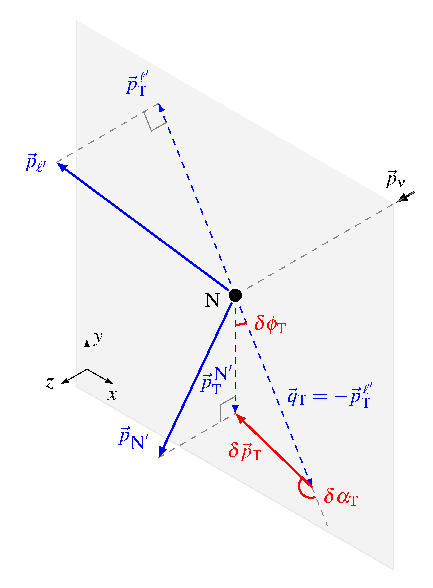
\includegraphics[width=0.35\textwidth]{figures/stki.eps}
    \caption{\label{fig:stki} Schematic illustration of the TKI variables. Diagram taken from Ref.~\cite{Lu:2015tcr}.} 
\end{figure}
In the simplest case, there are only two final particles after the neutrino-nucleon interaction, a muon and a proton. 
In the absence of nuclear effects, the muon and the proton should be emitted with momenta of the same magnitude but opposite direction in the plane transverse to the neutrino direction.
The TKI variables are constructed to quantify the deviation from this ideal scenario in measurements to access the nuclear effects. 
The presence of IS will affect the initial nucleon momentum, so the sum of the muon and proton transverse momenta will deviate from zero, which is quantified by $\dpt$, and their direction will not be exactly opposite, which is quantified by $\dphit$.
Furthermore, if the nucleus is assumed to be at rest and no other particles are knocked out other than the muon and the proton, the initial nucleon momentum, $\pn$, can also be estimated following the steps outlined in Ref.~\cite{Furmanski:2016wqo, Lu:2019nmf}. 
This esimation amounts to an approxiate  $\mathcal{O}(20\%)$ correction~\cite{Yang:2023dxk}. 
Hence, $\dpt$ and $\pn$ serve as good probes for IS models.
FSI will smear these distributions, but the shape and the peak position is mostly due to IS modelling.
All current IS models do not have a preferential direction for initial nuclear motion, so it is natural to assume the nucleons move in random directions isotropically, leading to a uniform $\dat$ distribution, which is the angle between the initial nucleon momentum and the proton momentum in the tranvserse plane. 
Thus, the deviation from flatness for $\dat$ can only be due to FSI, thereby making it an excellent probe for FSI. 
 
In the case of pion production, an additional doouble transverse variable, $\dptt$, can be constructed by projecting $\vecdpt$ onto the direction perpendicular to the lepton scattering plane, which is defined as the plane containing $\vecpl$ and $\vecpnu$.
The reconstruction is illustrated in Fig.~\ref{fig:dtki}.
\begin{figure}
    \centering
    \includegraphics[width=0.35\textwidth]{figures/dptt.pdf}
    \caption{\label{fig:dtki} Schematic illustration of the double TKI variable, $\dptt$. Diagram taken from Ref.~\cite{T2K:2021naz}.}
\end{figure}
In the absence of nuclear effects, $\dptt$ should be zero.
The spread of the $\dptt$ distribution is sensitive to the nuclear effects in pion production~\cite{MINERvA:2020anu, T2K:2021naz}.
Its equivalent in pionless production, $\dptx$, has been proposed and studied together with its orthogonal companion, $\dpty$, in MINERvA~\cite{MINERvA:2019ope}.
Additionally, Ref.~\ref{Lu:2015tcr,Hamacher-Baumann:2020ogq} suggests the possibility of using $\dptt$ to select a $\nu$-H sample.
Further details on a hydrogen sample selection will be discussed in Sec.~\ref{sec:tki-h}.

There has been a wealth of measurements from various neutrino experiments such as  T2K~\cite{T2K:2018rnz, T2K:2021naz}, MINERvA~\cite{MINERvA:2018hba, MINERvA:2019ope, MINERvA:2020anu, MINERvA:2021csy}, and MicroBooNE~\cite{MicroBooNE:2022emb, MicroBooNE:2023cmw, MicroBooNE:2023tzj, MicroBooNE:2023wzy, MicroBooNE:2024tmp}.
As the TKI idea is equally applicable to electron scattering, experiments such as CLAS~\cite{CLAS:2021neh} has also produced TKI measurments, showcasing the efficacy and wide applicability of TKI. 


% This document introduction won't serve as a complete primer on \LaTeX.  There are plenty of those online, and googling your questions will often get you answers, especially from \url{http://tex.stackexchange.com}.

% Instead, let's talk a little about a few of the features and packages lumped into this template situation.  The \verb|savequote| environment at the beginning of chapters can add some wittiness to your thesis.  If you don't like the quotes, just remove that block.

% For when it comes time to do corrections, there are two useful commands here.  First, the \verb|mccorrect| command allows you to highlight a short correction \mccorrect{like this one}.  When the thesis is typeset normally, the correction will just appear as part of the text.  However, when you declare \verb|\correctionstrue| in the main \verb|Oxford_Thesis.tex| file, that correction will be highlighted in blue.  That might be useful for submitting a post-viva, corrected copy to your examiners so they can quickly verify you've completed the task.

% \begin{mccorrection}
% For larger chunks, like this paragraph or indeed entire figures, you can use the \verb|mccorrection| environment.  This environment highlights paragraph-sized and larger blocks with the same blue colour.
% \end{mccorrection}
